\documentclass[11pt, a4paper]{article}
\usepackage[utf8]{inputenc}
\usepackage[italian]{babel}
\usepackage{geometry}
\geometry{a4paper, margin=2.5cm}
\usepackage{hyperref}
\usepackage{titlesec}
\usepackage{enumitem}
\usepackage{graphicx}

\title{Relazione di Progetto: Bomberman \\ \large Sezione: Gestione Livelli, Rendering e Statistiche}
\author{Prima parte(capitoli da 1 a 4) a cura di: \textbf{Bernardi Matteo Matricola: 0001211525}}
\date{}

\begin{document}

\maketitle

\section*{1. Architettura dei Livelli e Strutture Dati}
Una delle sfide principali nello sviluppo del progetto è stata la gestione dinamica degli stage di gioco. Ho optato per una netta separazione delle 
responsabilità dividendo la logica in due classi distinte: \texttt{Map} e \texttt{Level}.

\subsection*{1.1 Le classi Map e Level}
La classe \texttt{Map} gestisce esclusivamente i dati statici e spaziali del gioco. Si occupa di caricare la matrice bidimensionale da un file di testo 
diverso per ogni livello, verificare la validità dei movimenti tramite il metodo \texttt{isWalkable()} e identificare la presenza di ostacoli fisici (muri indistruttibili e blocchi distruttibili).
Inoltre in essa è presente il metodo \texttt{stamp\_map} il quale si occupa, per ogni ciclo di gioco, di stampare a schermo tutte le informazioni del livello corrente.
La classe \texttt{Level}, invece, funge da vero e proprio "Game Manager" per la singola istanza del livello. Al suo interno vengono gestite le entità dinamiche: 
il giocatore, i nemici, i potenziamenti (Item) e lo stato della bomba. Per garantire varietà nel gameplay, il costruttore di \texttt{Level} è stato 
implementato tramite overloading, permettendo di implementare livelli con combinazioni variabili di nemici e, di conseguenza, poter aumentare gradualmente la difficoltà di ogni livello.

\subsection*{1.2 Transizione tra i livelli: BidirectionalList}
Per ricreare un'esperienza cotninua e scorreevole, il passaggio tra i vari schemi non è lineare ma bidirezionale. A tale scopo è stata implementata 
una \texttt{BidirectionalList} custom. Questa lista doppiamente concatenata mantiene in memoria lo stato dei livelli generati:
\begin{itemize}
    \item Calpestando la cella Uscita (\texttt{'U'}), il giocatore avanza al nodo successivo, spawnando alle coordinate dell'Entrata (\texttt{'@'}) della nuova mappa.
    \item Calpestando l'Entrata (\texttt{'@'}), la lista retrocede al nodo precedente, permettendo di tornare al livello precedente (a meno che non sia gia stato completato) senza perdere i progressi (come i muri già distrutti).
\end{itemize}

\section*{2. Level Design (Da Excel a Testo)}
La progettazione dei livelli ha richiesto uno strumento visuale che permettesse di bilanciare rapidamente i percorsi e la densità dei muri. 
Si è scelto di utilizzare Excel, dove ogni cella rappresentava una cella del terminale. Tramite l'utilizzo di funzioni 
 di concatenazione stringhe (come \texttt{TESTO.UNISCI}), le matrici visive sono state 
esportate in file \texttt{.txt} formattati in modo rigoroso, preservando gli spazi vuoti calpestabili e prevenendo errori di 
lettura (come i ritorni a capo) durante la fase di I/O nel costruttore di \texttt{Map}.
\begin{figure}[htbp]
    \centering
    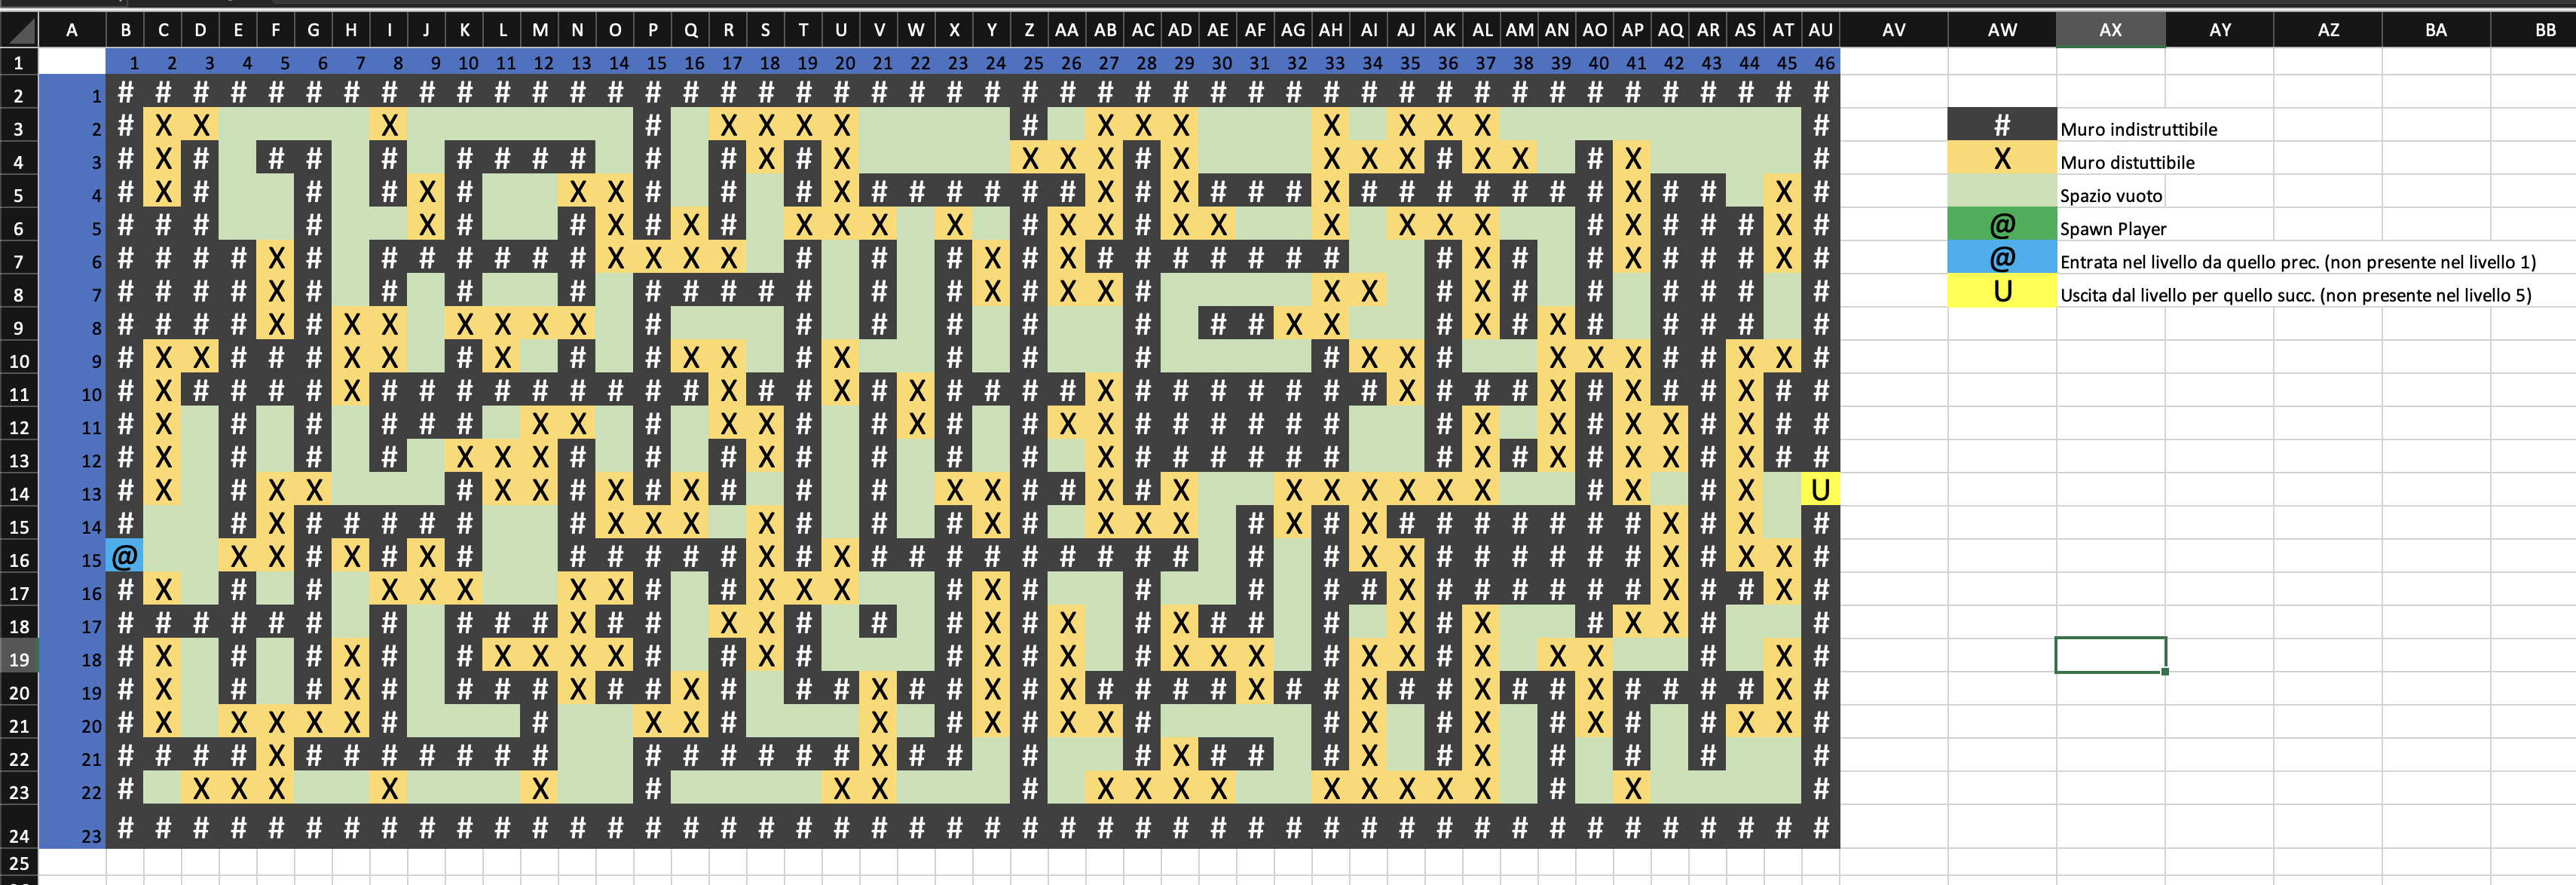
\includegraphics[width=0.85\textwidth]{img_relazione1.png}
    \caption{Progettazione del livello 4 su foglio di calcolo.}
    \label{fig:mappa}
\end{figure}

\section*{3. Rendering Terminale e Statistiche}
Tutta l'interfaccia grafica è stata realizzata sfruttando la libreria \texttt{ncurses}. 

\subsection*{3.1 Gestione delle Finestre}
Il rendering della mappa avviene su una finestra dedicata (\texttt{WINDOW* win}), circondata da un box estetico che viene dinamicamente "bucato" in 
corrispondenza delle porte per creare un effetto visivo di continuità.


\subsection*{3.2 Statistiche Laterali}
Al fine di fornire al giocatore tutte le informazioni vitali senza inquinare la matrice di gioco, è stato sviluppato un 
pannello laterale per le informazioni. Utilizzando 
le coordinate dinamiche (larghezza della mappa corrente + offset), la funzione \texttt{stampInfo()} 
renderizza in tempo reale le vite, il punteggio del giocatore, il tempo rimanente 
formattato (formato \texttt{MM:SS}) e un tracciamento in tempo reale della durata dei potenziamenti 
attivi (Boost Danno, Raggio, Timer). Sono state prestate particolari attenzioni all'uso 
corretto dei \texttt{COLOR\_PAIR} in combinazione con lo sfondo predefinito del terminale, e alla formattazione 
a larghezza fissa (es. \texttt{\%-4d}) per 
prevenire residui grafici durante i decrementi numerici.

\section*{4. Integrazione dei Large Language Models (LLM)}
L'utilizzo degli LLM è stato impiegato come strumento di debugging e problem-solving mirato. 
Non è stato generato codice intero, ma si è richiesto il supporto per:
\begin{itemize}
    \item \textbf{Debugging :} Comprensione e risoluzione di errori di linking (es. \texttt{symbol(s) not found for architecture arm64}) dovuti a 
        incongruenze di dichiarazioni tra file \texttt{.hpp} e \texttt{.cpp} della rispettiva classe, o alla propagazione del qualificatore \texttt{const} nel passaggio per riferimento di 
        oggetti complessi (come le istanze di \texttt{Bomba} o \texttt{Giocatore}).
    \item \textbf{Ottimizzazione di ncurses:} Consultazione della documentazione per risolvere le peculiarità della libreria grafica, 
        dalla corretta sequenza di refresh delle finestre alla manipolazione degli spazi vuoti in fase di rendering, fino alla gestione sicura dei colori di 
        default tramite \texttt{use\_default\_colors()}.
    \item \textbf{Esportazione mappe (Excel $\rightarrow$ txt):} Supporto nella stesura delle formule Excel necessarie per automatizzare la conversione sicura della 
        mappa da matrice tabellare a file di testo, gestendo la sostituzione delle celle vuote con singoli spazi calpestabili.
\end{itemize}

\end{document}